\documentclass[runningheads]{llncs}

\usepackage{amssymb}
\setcounter{tocdepth}{3}
\usepackage{graphicx}

\usepackage{url}
\newcommand{\keywords}[1]{\par\addvspace\baselineskip
\noindent\keywordname\enspace\ignorespaces#1}

\usepackage{url}
\urldef{\mails}\path|{david.pastor, yves.raimond, samer.abdallah, mark.sandler}@elec.qmul.ac.uk|

\begin{document}

\mainmatter

\title{A Logic-Based Framework for Digital Signal Processing}

\titlerunning{A Logic-Based Framework for Digital Signal Processing}

\author{David Pastor\and Yves Raimond\and Samer Abdallah\and Mark Sandler}

\institute{Centre for Digital Music, Queen Mary, University of London,\\
\mails}

\maketitle


\begin{abstract}
In this paper we describe a logic-based framework for Digital Signal Processing. This framework is implemented as a set of SWI-Prolog modules developing interfaces to heterogeneous signal processing libraries. A set of functors capturing common datatypes and a standard format for binary data are used to mediate our different analysis components. The system provides the user with a unified and flexible front-end to define signal processing workflows. The framework develops a signal processing-enabled reasoner capable of performing the primary tasks through the interfaces: decoding (specific libraries for each format), feature extraction (Vamp plugins), audio processing and effects (LV2/LADSPA plugins) and classification (WEKA machine learning API).

\keywords{Digital Signal Processing, SWI-prolog modules, signal processing workflows, processing-enabled reasoner, interfaced open source engines}
\end{abstract}

\section{Introduction}\label{sec:intro}

Digital signal processing (DSP) is a broad field and an important object of engineering research. Within this research community, particular investigators are discovering and developing new algorithms for signal processing and analysis. Many projects aim at developing formal APIs providing a framework for algorithms implementation. However, these APIs are normally designed as a closed environment which hardly interacts with other related APIs and applications. Although several APIs are wrapped and exported as ``plugin'' libraries which can be embedded in different applications, they still require the implementation of specific and non-interactive hosts.

This situation leads to many isolated applications, environments and sources of data working independently from each other. Any effort to combine them to obtain integrated results for analysis, classification and comparison requires tedious studies or ``glue code'' implementations.

In this paper we address this problematic situation by proposing and developing SWI-DSP, a logic-based framework for \textit{Audio Processing} (as subset of DSP) that extends the SWI-Prolog \cite{swi} vocabulary. We rely on a logic programming language with aggregated audio analysis capabilities getting rid of the application-dependency paradigm and offering a single logic front-end. Logic resources are also used to achieve a more capable DSP engine. The main and primary motivation for a logic-based implementation of such a system is to turn our conception of traditional procedural applications for computation of data towards semantic frameworks to manage knowledge involving specific computations.

In \S 2 we identify the most common audio analysis tasks and summarize several relevant \textit{open source} APIs aimed at performing such tasks. We evaluate the advantages and limitations of these APIs in order to find the requirements for SWI-DSP. In \S 3 we start viewing the system from the top and how it defines an interesting workflows-based architecture that characterizes input/output relationships between task-oriented modules. These workflows are possible by means of common functors and a binary data standard format. \S 4 goes into the implementation of each task-oriented module that develops communication layers with dedicated audio processing libraries that are in charge of the actual computation and offer an open development framework.

Thus, SWI-DSP extends SWI-Prolog vocabulary to perform audio analysis and processing by defining functors (capturing common datatypes) and predicates, triggering external computation performed by dedicated APIs, which are ordered in modules with different levels of abstraction. However, this architecture does not present an efficient and manageable framework as it requires specific module knowledge to create programs suitable for the concrete needs. We tackle this problem in \S 5 by defining an unified and flexible front-end, composed by DSP ``scenarios'', which allows the user to define workflows with understandable semantics.

Data management is an important paradigm involved in many domains and also in the multimedia research domain. Computations can not often be retrieved from session to session or are stored in local filesystems unlikely directed to extend any shareable source of knowledge because they are not expressed in a standard format with common semantics. This problem also encourages the approach presented in this work, based on a predicate calculus implementation (SWI-Prolog), in two different ways:

\begin{itemize}
 \item Concurrent Transcation Logic can be used to extend the predicate calculus to provide an unified logic framework for computations and data updating (given a database implementation).
 \item SWI-Prolog provides an important set of interfaces to other languages (to build user applications embedding the system) and packages that allow us to interact with semantic web technologies which seem to be the best framework to provide a common source of knowledge.
\end{itemize}

Although SWI-DSP does not develop a data management system itself, we discuss this problem in \S 6 and present related works which contribute to achieve such a multimedia knowledge reasoner/manager. We conclude in \S 7 by assessing the value and scope of this work and introducing future advances.

\section{Audio processing tasks and solutions}\label{sec:tasks}

A particular application of DSP is the study of one-dimensional, time domain signals that in real world often exist as audio signals. Audio signals evolve in time and have acoustic properties produced by the signal structure and shape. Music and speech are the main domains involving audio signals.

The properties of an analog and continuous signal (acoustic signals) can be studied by analysing their digital (sampled and quantified) versions. A one-dimension digital signal is therefore a processable sequence of values in a discretized time domain that represents the audio signal. Digital signals allow machine processing useful to modify the orignal signal or extract characterisitics from it. We can classify the digital signal processing paradigm in these main tasks:

\begin{itemize}
 \item Effects
 \item Feature Extraction
 \item Classification
\end{itemize}

\subsection{Effects}\label{subsec:effects}

A signal may be presented in a raw or non desirable way for its analysis so a basic stage of many systems is the pre-processing. The signal is processed to obtain a satisfying version of it by different techniques (filtering, normalization, amplification...).

It is very common in applied systems to provide tools that modify acoustic properties of the signal by introducing specific effects. Reverberation, delay or distortion are examples of effects that can be digitally obtained reproducing natural or instrumental alterations of the signal.

In practice, we can characterize this group of tasks for its input/output relationships. The operation outputs a signal (which may be time, frequency or multidimensional domain) when is fed with an input signal (accepting several domains as well). Oscillators and synthesis systems outputs signals without input.

One important dedicated API is the Linux Audio Developer's Simple Plugin API (LADSPA) \cite{ladspa}  which has been succesfully used in many systems and applications and is a widely spread implementation for algorithms development. We host LADSPA in SWI-DSP but there are other interesting libraries like DSSI plugins for effects and LV2 (new generation of LADSPA) which are targets for future extensions. 

\subsection{Feature Extraction}\label{subsec:feature}

Acoustic properties which are the substract of the psychological perspecitve of audio signals are conveyed in the signal and therefore in their digital representations. The so-called feature extraction paradigm aims at extracting different levels of audio features to characterize, classify and compare the audio signals (and any signal in general). The domain of the feature represents a qualitative side of the signal (tempo, chromatism, timbre...), so features do not convey all the signal information. This is interesting as distinct signals may have some very close features and differ much in others.

The Vamp Plugins API \cite{vamp} offers a framework to develop feature extraction plugins that can be hosted in any application able to control the ``plugin lifecycle''. We host Vamp plugins as basis for feature extraction in SWI-DSP. In general plugin libraries are characterized for being suitable for development but application-dependent.

\subsection{Integrative solutions}\label{subsec:inte}

With the same motivation of this work there are some integrative APIs which combines different tasks to perform low and hig-level operations in a closed implementation. CLAM \cite{clam}, jMIR \cite{jmir} and Marsyas \cite{marsyas} present a complex framework collecting tools to perform different DSP tasks. The most interesting feature of these frameworks is the possibility to create DSP networks combining specific algorithms and modules thanks to a workflow-based architecture (Marsyas and CLAM) or with a descriptive task format (jMIR).

CLAM also offers a metamodel of DSP processes wich provides semantics to design the networks properly presenting a higher and more manageable level of abstraction. However, these APIs still present two important limitations that our work is aimed at solving:

\begin{itemize}
 \item They do not offer a common format to exchange data or an easy way to interact with other applications.
 \item They are based on a procedural system unable to reach higher-level knowledge by itself.
\end{itemize}

\subsection{Classification}\label{subsec:classif}

Classification is one the most interesting and complex paradigms in any specific domain exploiting the ``intelligence'' of computational machines. WEKA (Waikato Environment for Knowledge Analysis) \cite{weka} collects different machine-learning algorithms and provides several user interfaces to manage the analysis. It aslo provdes a formal interface (in Java) for development and interaction with other systems.

However, this generic API does not provide semantics to create a dataset which is the most intriguing and complex issue for classifying data properly. Marsyas and jMÍR integrate WEKA orienting it for music classification purporses by offering a code interface with other modules (Marsyas) or by extending the WEKA file format ARFF (jMIR). Both solutions still seem to lack of effective semantics and a interactive front-end to perform classification of audio data.

\section{SWI-DSP architecture}\label{sec:architecture}

From the previous comparison and review we consider that a innovating system should satisfy the following requirements:

\begin{itemize}
 \item Allowing workflows design
 \item Providing an interface to interact with other related systems and applications
 \item Featuring an unified, flexible, interactive and understandable front-end
 \item Providing an open-development platform
 \item Management of shareable data semantically labelled
 \item Enhancing traditional procedural implementations by building a logic-based framework of declarative nature allowing reasoning and inferencing.
\end{itemize}

As initial step, we build a framework able to develop digital signal processing workflows based on a predicate logic implementation (SWI-Prolog) extending its vocabulary by wrapping computations under logic predicates. We develop task-oriented modules and define functors capturing the common datatypes allowing the communication between modules and hiding the internal implementation. In addition to this, we define a standard format for binary data ``spoken by every SWI-DSP module''. We define these utils in the \textbf{swilib} module which provides a C++ library and a SWI-Prolog module for their management.

This layout allow us to wrap fast and efficient implementations of algorithms (in some imperative language) to provide predicates that determine the relationship between defined types (as black box computation) giving a ``functional programming'' view of the system preserving computational efficiency. This functional programming approach (which allow us to create workflows as rules with a procedural meaning) is motivated by the advantages of functional languages like Haskell \cite{haskell} that present a semantically oriented view of computations instead of a machine-oriented one. There are also several works that develop such a typed-functional language on a logic framework like lambda-Prolog \cite{lambda} or Mercury \cite{mercury}. However, our approach results to be more suitable to develop an open platform for research and development. External engines based on open source APIs provide faster computations than any functional or logic/strong-typed language and a suitable developers interface. Furthermore, SWI-Prolog features a very powerful, interactive and flexible front-end which is also a requirement for the proposed system.

\subsection{Datatypes controlling workflows}\label{subsec:datatypes}

In section \ref{sec:tasks} we have seen how tasks are strongly characterized by their input/output relationship. The system requires datatypes that guarantee the correct input and output matching. We identify these datatypes by analysing the tasks classification. We also want to look at the Music Ontology specification \cite{mo} as a ``web ontology'' description of music-related concepts including audio analysis terminology. We distinguish the following datatypes:

\begin{itemize}
 \item signal: this type represents an audio signal in a physical timeline. 
 \item feature: this type represents some side of the audio signal properties
 \item parameter: this type represents the different variables of the computation context (computations are not only a one-to-one function)
 \item timestamp: this type represent the reference of a data object to a timeline
\end{itemize}

We implement these datatypes in SWI-Prolog as functors (name/arity) that bind together the attributes of a concept (e.g. signal(Channels, SampleRate, Length, [DataIdPerChannel])). These datatypes (with the disadvantage of being a non-flexible model) can be interpreted by any module guaranteeing the correct instantation pattern of the predicates and ensuring a valid execution.

\subsection{Large Binary Objects}\label{subsec:blobs}

Large binary data is present in any multimedia system and needs to be treated in the most efficient and manageable way. The so-called BLOBs are objects wrapping large binary data. The representation of data in SWI-Prolog can be done through lists which can not handle such amount of data (e.g. signals of 1000000 samples) or through SWI-Prolog BLOB terms which are cumbersome as datatype.

We have implemented a mechanism of \textit{data identifiers} that vary incrementally and are stored in a database updated in each session. Each identifier holds the binary representation of an arbitrary large sequence of floating point format data. This identifiers-based system is useful in the following ways:

\begin{itemize}
 \item It hides awkward binary representations or inefficient SWI-Prolog lists by handy representations of data as atoms: e.g. \textbf{\_\_data\_435}
 \item It implements a look-up database whose status can be easily updated and checked
 \item It provides multiple ways to export/import data to the database through the identifiers. Data can be wrapped into or extracted from a blob term, displayed/read as prolog list (length restrictions) and dump into or load from a binary file
 \item It unifies the ``raw'' data representation allowing the communication at the lowest level between modules 
\end{itemize}

The following example shows how a decoded audio file can be easily represented by the data identifiers that make easy to work with such a big sequence of data.
\begin{verbatim}
?-decode('../myfile.*', Signal).
Signal = signal(2, 44100, 1200000, ['__data_0', '__data_1']).

?-data_out('__data_0', '../myfilech1').
?-data_out('__data_1', '../mufilech2').

?-get_frame(signal(2, 44100, 1200000, ['__data_0', '__data_1']), 200, 5,
frame(Ch, Sr, L, [Ch1D, Ch2D])),
data_to_list(Ch1D, List), length(List, Llen).
Ch1D = '__data_2'
List = [6.45, 4.56, 3.23, 9.78, 3.26]
Llen = 5
\end{verbatim}

\subsection{Processing workflows}\label{subsec:worflow}

\begin{figure}
\centerline{\framebox{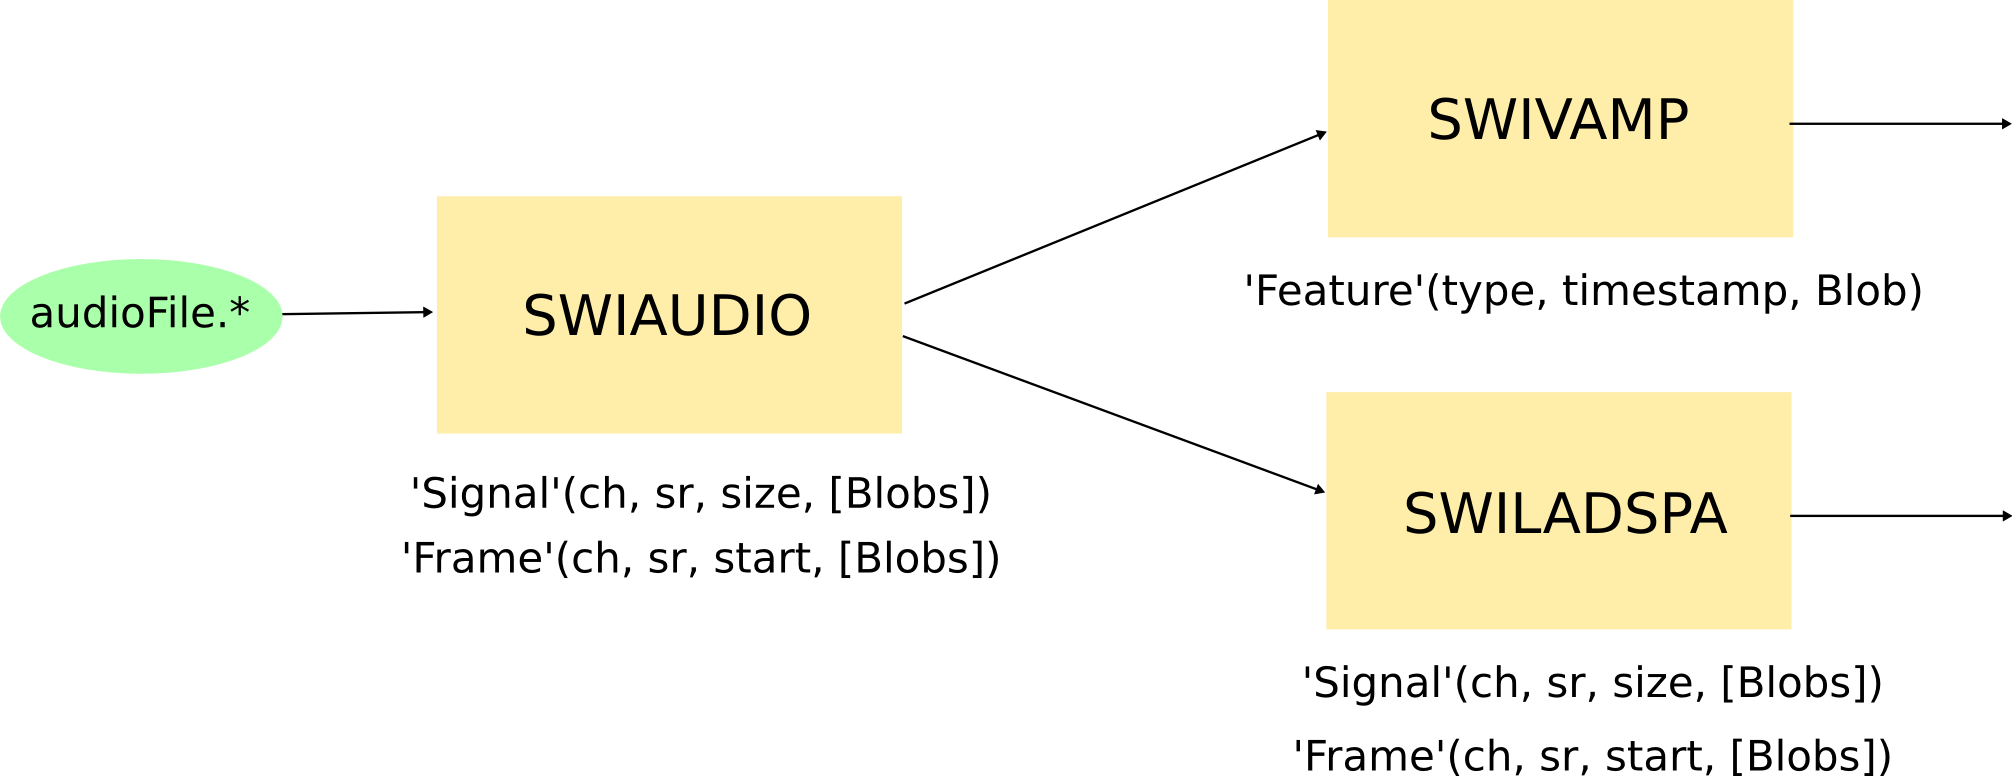
\includegraphics[width=\columnwidth]{workflow.png}}}
\caption{Example of how to create a workflow: compare the tempo of a signal and a reverbered version of it}
\label{fig:workflow}
\end{figure}

Figure \ref{fig:workflow} shows a possible workflow that is designed by using the functional framework formed of datatypes, a standard format for data and the modules of SWI-Prolog predicates which are described in \ref{sec:modules}.

\section{SWI-DSP modules}\label{sec:modules}

Each task (functional) module is composed by lower level modules which offer communication with an external API or library in charge of the computations. By hosting ``plugin libraries'' we can extend easily the SWI-DSP vocabulary (new plugins can be added without code modifications).

\subsection{swiaudio}\label{subsec:swiaudio}

This module is in charge of providing audio data to the system. This module is splitted in two sub-modules: \textbf{swiaudiosource} and \textbf{swiaudiodata}. The former is a powerful module for decoding which interacts with C decoding libraries (mad, soundfile, fishsound, oggz and faad) to extract a \textit{Signal} term given and audio input file supported by the libraries. This process is triggered by a simple call to the predicate \textit{aspl\_decode(+InputFile, -Signal)} which recognizes the file extension and calls a specific library allowing a fast decoding process and even more important an independent term representing the encoded data in a standard way for any format.

The latter is a module which defines utilities typically required in DSP. The most important set of predicates is dedicated to framing. The original signal is decomposed in overlapping blocks of data outputting frame terms through the non-deterministic predicate \textit{framing(+Signal, +StepSize, +BlockSize, -Frame)}. This predicate calculates the number of possible frames using the length of the Signal and the StepSize and creates a list of natural indexes which are passed to the low-level framing predicate in a non-deterministic way using member/2. The rest of predicates are mainly oriented to extract information from a Signal or Frame term.

\subsection{feature extraction}\label{subsec:swivamp}

This module defines a standard task-oriented set of predicates for feature extraction. As we have seen in \S 2 the module is characterized for a clear input/output relationship. So we can declare a simple predicate to extract the tempo of an audio signal: tempo(+Input, -Tempo) being Input an instantation of the Signal datatype and Tempo a list of instantations of the Feature datatype. This predicate that returns a tempo-related list of features given an input signal is indeed triggering a specific computation tool, so we could select the specific tool by extending the predicate: \textit{tempo(+Input, +Tool, -Tempo)}.

We rely on the Vamp Plugin API as it offers an efficient plugin and host implementation. Certainly, there is a limitation in the sense that any feature extraction algorithm we may want to use has to be implemented as Vamp Plugin, but as counterpart it is easier to write an algorithm as Vamp Plugin than to interface many APIs or particular algorithm implementations.

The sub-module \textbf{swivamp} is a communication layer based on the SWI-Prolog foreign interface which allow us to query the plugin information, set up the plugin context for the transform, execute the plugin given a Signal term and retrieve the output features for the plugin according to the lifecycle specification. Plugins are wrapped in a similar fashion than the audio data so we can use a plugin instance representation which allow us to have concurrent plugins working at the same time. The previous tempo/3 predicate is declared as this set of rules:

\medskip

\noindent

\begin{verbatim}

tempo(Input, Tool, Tempo):-
     Input = 'Signal'(Ch, Sr, L, PCMs),
     Tool = 'Vamp',
     vamp_feature_of('tempo', Signal, WholeFeature).
vamp_feature_of(Type, Signal, WholeFeature):-
     select_plugin(Type, PluginKey, Output),
     vamp_outputs_for(Signal, PluginKey, Output, Features),
     flatten(Features, WholeFeature).
vamp_outputs_for(Signal, PluginKey, Output, Feature):-
     vmpl_load_plugin_for(PluginKey, Signal, Plugin),
     set_blockSize(Plugin, Block),
     set_stepSize(Plugin, Step),
     get_channels(Signal, Channels),
     vmpl_initialize_plugin(Plugin, Channels, StepSize, BlockSize),
     vamp_compute_feature(Signal, Step, Block, Outputs, Plugin, WholeFeature).
vamp_compute_feature(Signal, Step, Block, Outputs, Plugin, Features):-
     get_samples_per_channel(Signal, L),
     findall(F, vamp_process_signal(Signal, L, Step, Block, Output, Plugin, F), FSet),
     get_sample_rate(Signal, SampleRate),
     vmpl_remaining_features(Plugin, L, SampleRate, Outputs, Remaining),
     append(FSet, Remaining, RawFeatures),
     delete(RawFeatures, [], Features).
vamp_process_signal(Signal, L, StepSize, Block, Out, Plugin, Features):-
     set_limit_framing(L, StepSize, Limit),
     set_framing(StepSize, L, Limit, Start),
     vmpl_process_block_framing(Plugin, Signal, Start, Block, Out, Features).

\end{verbatim}
\noindent

\subsection{audio processing}\label{subsec:swilasdpa}

This module defines any computation which outputs a Signal term. It comprises any sort of effect or filtering over a signal. It reproduces a real time processing by outputting processed frames as they are computed (non-deterministic call to a processing predicate) or stores the processed blocks to return and altered version of the input signal. 

The module swiladspa offers communication with LADSPA which is the most generic and spread plugin API for general audio processing. The communication layer allows us to query the plugin description, control the set up of the plugin (control and audio ports) and retrieve the processed data. Through predefined routines we can offer a more handy access to the plugin or even declared predicates just defined by an input/output relationship.

\subsection{swiweka}\label{subsec:swiweka}

The WEKA API is interfaced through the package JPL available for SWI-Prolog defining a complex Java-Prolog interface to read/write ARFF files, load ARFF files, instantiate classifiers, execute classification and retrieve the classification scores of the dataset. This communication layer offers a really cumbersome and API-dependent module which requires semantics and interpretation rules to become into a useful logic-framework for audio data classification as described in the next section.

\section{DSP front-end}\label{sec:frontend}

So far we have presented how SWI-DSP provides a vocabulary of logic predicates and datatypes to perform audio analysis imitating a functional language, but this aproach is still inappropiate for such tasks. We have organized the modules in communication layers and task-oriented modules, but there is an important trade-off between understandability and specification. The communication layer even offering an application-independent access to the computation libraries still requires a high knowledge of such libraries besides a SWI-Prolog familiarization which is not expected in most part of the potential users. The datatypes are not the only necessary semantic resource to provide an actual workbench for DSP. We require a front-end that reflects the experimental domain providing an interactive ``laboratory''.

We define some ``DSP scenarios'' that reflect the researching activity. This scenarios define the necessary patterns and datatypes (implemented as predicates and functors) to allow the user to actually perform high-level research preserving the necessary flexibility. The elemental scenarios are:

\begin{itemize}
 \item Transform: This scenario provides a pattern to apply any computation over an audio signal. It specifices by a datatype the framing parameters, the running engine, the engine configuration and parameters, the sample rate (if variable), the type of transform and the domain specifications. These factors are captured with a functor used to link input/output (with full flexibility) in transform(+Input, +Transform, -Output)
 \item Classification: This scenario is provided for a proper setup of classification. This scenario specifies the classification domain, the categories (names, types and ranges), the classification schema and the training set. It also provides a pattern for the input data set which is interpreted along with the classification environment to return the resulting 
\end{itemize}

The patterns and functors are interpreted by hardcoded prior knowledge which starts up the subsequent steps to provide the queried output. More complex scenarios can be created in order to achieve higher or broader semantics for research activity. This interactive logical framework can be interfaced, tranlasted or embedded into other environments by means of the wide range of SWI-Prolog tools (see \ref{subsec:henry}).

\section{Data management and computation reasoning}\label{subsec:datamanage}

We still need to address, probably, the most important issue to accomplish the proposed architecture. We could say that such a system is indeed aimed at managing complex and large data, which is related through computational ``blocks'', and allowing reasoning about it. This goal requires the following achievements: an efficient storage of data objects and the relationships (predicates) linking them, mechanisms to control the concurrency, consistency and side-effects of the computations and a high-level interface to interact with them.

We do not develop such manager within SWI-DSP as the database implementation actually depends on the needs of the host agent interacting with SWI-DSP. However, supposed a database we can describe the architecture in detail. Data is stored in the database by ``tabling'' predicates (which link the input, the context and the output). Tabled predicates (we table predicates that comprise a big load of computations) are stored in the database the first time they are called so data can be retrieved automatically without running the external engines simulating not functional but semantic relationships of complex (audio) data. For this purpose, the data identifiers mechanism seems to be ideal as data ids are linked (and binary data is dumped and loaded from external files relieving memory) and stored wraping complex data as a declarative-oriented units of knowledge. An example of a tabled predicate is:

\begin{verbatim}
?-table(decode('../myfile', signal(2, 44100, 1200000, ['__data_345', '__data_346']))).
\end{verbatim}

Our functional-view system can be seen now as a knowledge source that can be managed by combining procedural declarations of execution paths and declarative transactions and updates of data by means of Concurrent Transaction Logic.

\subsection{Concurrent Transaction Logic}\label{sec:ctl}



\subsection{Henry}\label{subsec:henry}

Although SWI-Prolog is a well-known and used implementation of Prolog it does not represent the most suitable framework to deal with multimedia data. The multimedia community in general needs a standard machine-readable format with proper semantics to manage data. The Resource Description Framework (RDF) has been proposed as such a format and defines an Standard to represent linked data by means of triples in the form of (Subject, Predicate, Object).

This standard can be implemented with different syntaxes. We prefer to use Notation3 [x] whose syntax allow us to write RDF statements in a human-readable way and also to write ``rules'' as named graphs [g]. This is a suitable framework to represent data that can be shared and published in the so-called ``web of data``.

The Ontology Web Language (OWL) provides the framework to express the knowledge of a particular domain in RDF through concepts and relationships. Thus, descripting semantic models related to audio analysis are not restricted to a local implementation but can be shared and processed by different systems.

The project called Henry implements an N3/Prolog parser and reasoner based on Concurrent Transaction Logic. This agent defines an entailment module capable of reasoning over the SWI-DSP computations, which are identified through Universal Resource Identifiers (URIs), and N3 statements and rules. The semantic web package module for SWI-Prolog interprets SPARQL queries which are passed to Henry which produces RDF descriptions of computations by performing the entailment and triggering SWI-DSP computations.

\subsection{Visualisation}\label{subsec:vis}

Audio data can just be poorly interpreted in a float/binary format. Time and frequency domain signals and features in other domains are meaningful for an expert when they are visually represented. Although a logic domain does not seem to be the perfect environment to visualise audio data, we can easily save this difficulty. 

By controlling SWI-DSP by means of Henry we can easily convert our Prolog types and binary data into RDF (machine-readable) descriptions where each source of data is represented through a link or as a ''literal`` in a basic datatype format. RDF descriptions can be easily browsed with the new extensions of classical web browsers for linked data. Even more interesting, dedicated agents with an SPARQL point are able to query DSP through the semantic web resources as explained in \ref{subsec:henry}. Thus, we are able to visualise our own computations but also a scalable web of data with shared semantics which is enriched with computations from other local machines.

(I dont know if i should mention SV and the new extensions here....)

\section{Conclusion and Future work}\label{sec:conclusion}

We have presented a powerful reasoner for multimedia analysis implemented as a logic-based framework which allow us to convert low-level computations into shareable and distributed knowledge. The system design ''breaks apart`` traditional applications architecture to introduce logic and reasoning machinery on top of the computation engines providing a more intelligent, capable and understandable DSP reasoner. This reasoner can be extended and enriched by the open source APIs working on the foundations of the system and controlled by ''Prolog-speaking`` agents. SWI-DSP is fairly well positioned for the new web technologies and actually it finds in them the perfect semantic and storing support to overwhelm traditional and closed DSP systems.

Future work and development is oriented to:

\begin{itemize}
 \item Testing and comparison of performance with other rival systems
 \item Extending the SWI-DSP vocabulary and capabilities
\end{itemize}

SWI-DSP vocabulary and cabalities can be extended in several ways. First, by interfacing more open source APIs to cover the implementation of any DSP task (not necessarily restricted to audio domain). Secondly, by supporting symbolic data (MIDI) input which is a really important source of audio knowledge and providing analysis modules for such an input. Finally, other logic paradigms can contribute to enhance SWI-DSP (e.g. there are studies that use Inductive Logic Programming systems to extract harmonic rules or rhythm patterns given certain input descriptors [ref]). By providing semantics (OWL ontologies cleary point to this goal) to interconnect properly each logical module we can build a hierarchy of modules which help us to extract and share different levels of knowledge from digital signals. Such a system could be used either to extract low level cepstral coefficients from an input signal (mathematics level) or to obtain patterns of music (musicology level).

\begin{thebibliography}{4}

\bibitem{distributed} Raimond, Y., Sutton, C., Sandler, M.: A distributed data space for music-related information. In: Workshop on the Many Faces of Multimedia Semantic. ACM (Multimedia), Augsburg (2007).

\bibitem{ctl} Bonner, A.J., Kifer, M.: Concurrency and Communication in Transaction Logic. In: Joint International Conference and Symposium on Logic Programming, pp. 142--156. Bonn (1996)

\bibitem{tlprog} Bonner, A.J., Kifer, M.: Transaction Logic Programming. In: 10th International Conference on Logic Programming. Budapest (1993)

\bibitem{clam} CLAM, \url{http://www.clam.iua.upf.edu/}

\bibitem{marsyas} Music Analysis, Retrieval and Synthesis for Audio Signals. \url{http://marsyas.sness.net/}

\bibitem{jmir} McKay, C.: jMIR. \url{http://jmir.sourceforge.net/}

\bibitem{mo} Raimond, Y., Abdallah, S., Sandler, M., Frederick, G.: The Music Ontology. In: 8th International Conference of Music Information Retrieval. Vienna (2007)

\bibitem{kmrdf} Source code project of KM-RDF. \url{http://code.google.com/p/km-rdf/w/list}

\bibitem{ladspa} Linux Audio Developer Simple Plugin API. \url{http://www.ladspa.org/}

\bibitem{vamp} Cannam, C.: Vamp Plugins. \url{http://www.vamp-plugins.org/}

\bibitem{weka} WEKA home site \url{http://www.cs.waikato.ac.nz/ml/weka/}

\end{thebibliography}

\end{document}
